\documentclass[preprint,11pt,authoryear]{elsarticle}
%\documentclass[final,5pt,authoryear,twocolumn]{elsarticle}
%\usepackage[margins=1in]{geometry} 
%\usepackage[width = 5.5in, right=2.5in, marginparwidth=2.0in]{geometry} %adjusted to use todolist
\usepackage[margin=2.5cm]{geometry} %adjusted to use todolist
\usepackage{natbib}
\usepackage{graphicx}
\usepackage{epstopdf}
\usepackage{xcolor}
\usepackage{nomencl}
\usepackage{enumitem}
\usepackage{amsmath}
\usepackage{lineno}
\usepackage{framed} % Framing content
\usepackage{caption}
\usepackage{subcaption}
\usepackage{multirow}
\usepackage{longtable}
\usepackage{hyperref} % hyper referenceing
\usepackage{ftnxtra} % for foot notes
\usepackage{subcaption}
\usepackage{placeins}  % to force the bibliogrpahy to the end
\usepackage{listings}  % for python code syntax highlighting
\usepackage{colortbl}
\usepackage{multicol} % Multiple columns environment
\usepackage{mdframed}
\usepackage{todonotes} %add review notes
\usepackage{url}
\usepackage{courier}  %fixed width courier font
\usepackage{array}  % wrap text in the column 
\usepackage{soul}
\usepackage{tikz}
\usepackage{floatrow} % added this package for creating a figure beside a table
\usepackage{blindtext} % added this package for creating a figure beside a table
\usetikzlibrary{shapes,arrows}
\setlength{\nomitemsep}{-\parskip}
\renewcommand*\nompreamble{\begin{multicols}{2}}
\renewcommand*\nompostamble{\end{multicols}}
\graphicspath{{figures/}}

\newfloatcommand{capbtabbox}{table}[][\FBwidth] % added this command for figure and table side by side
\newcommand{\com}[1]{\todo{#1}} %short, popout comments
\newcommand{\lcom}[2]{\todo[inline, caption={#1}]{#2}} %long comments, keep inline, require short description
\newcommand{\icom}[1]{\todo[inline]{#1}} %short, inline, comments
%\setuptodonotes{disable} %uncomment to remove to-do notes from PDF, comment to add.

\newcommand{\mathcolorbox}[2]{\colorbox{#1}{$\displaystyle #2$}}

%\linenumbers %I'm not sure if you need to do this, I think their online system does this for you.
\journal{International Journal of Refrigeration}

\makenomenclature

\newcommand{\nomunit}[1]{%
\renewcommand{\nomentryend}{\hspace*{\fill}#1}}

\definecolor{mygreen}{rgb}{0,0.6,0}
\definecolor{mygray}{rgb}{0.5,0.5,0.5}
\definecolor{mymauve}{rgb}{0.58,0,0.82}

\lstset{ %
  backgroundcolor=\color{white},   % choose the background color
  basicstyle=\tiny\fontfamily{courier}, % size of fonts used for the code
  breaklines=true,                 % automatic line breaking only at whitespace
  captionpos=b,                    % sets the caption-position to bottom
  commentstyle=\color{mygreen},    % comment style
  escapeinside={\%*}{*)},          % if you want to add LaTeX within your code
  keywordstyle=\color{blue},       % keyword style
  stringstyle=\color{mymauve},     % string literal style
}


\newcolumntype{L}{>{\centering\arraybackslash}m{3cm}}  % wrap text in column
\begin{document}
%\blindtext % added this line for creating a figure beside a table

\begin{frontmatter}

\title{Evaluation and Quantification of Semi-Empirical Compressor Model Predictive Capabilities under Modulation and Extrapolation Scenarios}

\author[1]{Kalen S. Gabel\corref{cor1}
\fnref{cor1}}
\ead{kaleng@okstate.edu}
\author[1]{Craig R. Bradshaw}
\address[1]{Center for Integrated Building Systems, Oklahoma State University, Stillwater, OK 74078}
\cortext[cor1]{Corresponding author,Tel: +6206552222}
%\newpageafter{author}
\begin{abstract}

Testing and evaluation of select semi-empirical compressor models is carried out to quantify performance in modulation and extrapolation scenarios. Three representative models from literature are benchmarked against an artificial neural network (ANN) model and the industry standard AHRI model. A methodology for quantifying model performance, compared against experimental data, in extrapolation and modulation scenarios is presented. Predictions from the five models are compared against high-fidelity performance data taken from either a hot-gas bypass load stand or a compressor calorimeter. Scroll, screw, reciprocating, and spool compressor technologies collected with R410A, R1234ze(E), R134a, and R32 refrigerants. In total, 327 experimental data points were collected for model testing. The Mean Absolute Percentage Error (MAPE) is calculated for the mass flow rate and power of each compressor providing a mean to quantify the models ability to predict experimental data under modulation and extrapolation scenarios. [Add some quantification here of results, key results] The semi-empirical models yield MAPE’s less than 5\% for mass flow rate and power in modulation scenarios while performing at or below 8\% MAPE in envelope extrapolation scenarios. The semi-empirical models also capture superheat extrapolation to below 6\% MAPE for mass flow rate and power with the exception of one model [what model, name it] performing at 18\% MAPE in power prediction for one data set [what data set, name it]. The empirical formulations do not predict modulation behavior and showed varying performance at the extrapolation scenarios. Limitations with respect to model training data and overall performance are described. Future work includes the development of a new semi-empirical model will be developed, based on a semi-empircal formulation that can capture multiple compressor technologies while exhibiting good modulation and extrapolation capabilities.

\nomenclature{MAPE}{Mean Absolute Percent Error}
\nomenclature{ANN}{Artificial Neural Network}
\end{abstract}

\begin{keyword}
Semi-empirical compressor modeling \sep extrapolation \sep modulation \sep model evaluation
\end{keyword}

\end{frontmatter}

\clearpage
%make list of to-do's from comments, comment out to remove list
\listoftodos

\section{Introduction}

In 2020 the residential building sector in the United States used approximately 1.46 trillion kWh of electricity accounting for 39\% of total retail sales. Heating ventilation, air conditioning, and refrigeration (HVAC\&R) equipment consumed the largest percentage (37\%) of energy within this sector, \cite{EIA}. The compressor operating in a vapor compression cycle is the largest energy consumer in HVAC\&R systems, accounting for up to 80\% of system energy use [citation]. Today compressor manufactures are challenged by regulatory changes aimed at mitigating climate change and global warming, while still meeting system efficiency requirements. Modeling compressor performance is a vital part in estimating overall system behavior and mitigating excessive energy use.

\begin{framed}
\printnomenclature
\end{framed}

\lcom{}{I think this paragraph needs re-thought a bit. In my mind, you are motivating modulation and extrapolation capabilities of a model. You kind of touch on a few reasons for this here but none of them are 100\% clear to me.  I think you can focus on how regulatory changes are requiring manufacturers to design new product with higher efficiency standards, this creates need for high throughput of both simulation and testing and a model that enables prediction of part-load performance (modulation) and extrapolation will expedite that development.}When manufactures test their systems through simulation it is desired that a variety of operating conditions be predicted accurately. Additionally, part-load conditions sometimes require the compressor to be operated at a different operational speed \com{careful, modulation is broader than variable speed} than full-load conditions. These two situations present unique needs that a model must fulfil, that is, extrapolation and modulation capability. Semi-empirical models may have the potential of meeting these two needs. \com{I moved this section up, I think it is important to motivate the needs of a model first, then describe the model types}

Compressor models exist on a spectrum, ranging from black-box \com{I think it is helpful to hyphenate phrases like this} (statistical correlations) to white-box (distributed models). Black-box models require little information about the machine itself, while white-box models need detailed input information sometimes only known by the manufacturer. The most well known black-box model is the industry standard 10-coefficient map standardized by AHRI 540 \citep{AHRIstandard}. Grey-box or semi-empirical models aim to hit the middle ground between the two extremes. These models are more computationally efficient than white-box models and can be implemented into system simulations but include additional fidelity that black-box models typically do not. 


\lcom{re-organize this paragraph}{This section is way too much shoved together and is far too long for a single paragraph. I suggest going back through this and trying to organize it a bit into a few paragraphs that collect the most relevant work and presents it in a way that supports your narrative.  Given how you started the paper, I think it would be best to try and collect work based on the level of "`grayness"' they present, perhaps start from the most black-box of models and work toward white-box models. Each citation should support this directly, if it does not, consider if it needs to be included or not.  I also don't see any work on ANN's included here, it should be included since it was a selected model type. }This work aims to identify select semi-empirical compressor models from literature, quantify performance at extrapolation and modulation scenarios, and give insights into future model capable of predicting multiple compressor technologies in said scenarios.\cite{Li2012} gives a semi empirical method to calculate mass flow rate, shaft power, and discharge temperature using four different refrigerants and three types of variable speed compressors: reciprocating, scroll, and rotary. The author presents volumetric and isentropic efficiencies as second order functions of normalized speed, claiming the two may be independent of pressure ratio. For variable speed performance modeling, the method used a reference at a nominal frequencies to calculate volumetric flow rate at other speeds. The RMS error for the model is less than 3\% for mass flow rate and compressor power, while the discharge temperature RMS error is 3K. \cite{Li2012a} presented semi empirical model for hermetic scroll and reciprocating compressors with a focus on extrapolation. The model is able to capture mass flow rate, compressor power, and discharge temperature for reciprocating and scroll compressors with all the main parameters modeled within 5\% relative error. Compressor data is taken from other literature sources and extrapolation performance is tabulated in the study. Conditions where the saturated suction temperature is 10$^{\circ}$C or the saturated discharge temperature is 15$^{\circ}$C away from experimental data used for parameter fitting showed good accuracy, ~5\%. \cite{Navarro2007} presents a phenomenological model for analyzing reciprocating compressors using propane. The compressor efficiency and volumetric efficiency is presented as a set of implicit equations. The model needs 10 empirical parameters, each claimed to have physical interpretation, to be curve fitted. The computational time for fitting these parameters using a Monte Carlo method is lengthy. This model is supposed to be compatible with variable speed application. It reproduced compressor and volumetric efficiency with an error lower than 3\% under a wide range of operating conditions. \cite{Corber2007} use the model presented by \cite{Navarro2007} to predict reciprocating compressor performance with R407C and propane as the refrigerants. The work used parameters fitted with propane to estimate performance with R407C. Results showed deviations of less than 5\% for compressor efficiency in all tests except one. A phase change factor was adjusted in the model and results improved. \cite{Tello-Oquendo2019a} presents a semi-empirical model based on \cite{Navarro2007}'s work to predict scroll compressor performance. The method is extended to capture vapor injection scroll compressors using R407C, where results obtained were $\pm$ 5\% for compressor and volumetric efficiency. The suction mass flow rate, injection mass flow rate, compressor power and discharge temperature were reported with deviations lower than $\pm$ 2\%, $\pm$ 4\%, $\pm$ 5\%, and $\pm$ 4K, respectively. \cite{Mackensen2002} presented a semi empirical model for reciprocating, screw, and scroll compressors. The mass flow model is based on the concept of a polytropic process and volumetric efficiency. The polytropic process model is also used to predict power consumption. An efficiency factor was found to be necessary for the model and it is based on the operating conditions. The model had a maximum average mean weighted error of 3.7\%, 2.3\%, and 0.6\% for mass flow rate of the reciprocating, scroll, and screw, respectively. The model had problems with the power consumption estimates leading to an average mean weighted error of 8\%, 7.6\%, 6.4\%, and 5\% for the screw, scroll, open-drive reciprocating, and semi-hermetic reciprocating, respectively. \cite{Jahnig2000} presented a semi-empirical model for small hermetic reciprocating compressors used in household refrigerators. The model is based on volumetric efficiency and assumes a polytropic compression process. There are five parameters that must be determined by fitting experimental data. The authors find that the model extrapolates within 5\% error with condensing and evaporating temperatures that extend measured data by 10$^{\circ}$C. \cite{Shao2004a} presents a map based modeling approach for variable speed rolling piston compressors. The authors conclude that the ratio of mass flow rate at a constant frequency to that at the basic frequency remain constant at different evaporating and condensing temperatures. This observation is then used to define a mass flow rate ratio which is expressed as a second order function of compressor frequencies. A power ratio is defined similarly. Validation is done by comparing the model to experimental data yielding the maximum error to be 3\%, 5\%, 8\% and the relative error to be 2\%, 3\%, and 4\% for the refrigerant mass flow rate, compressor power, and COP, respectively. \cite{Aprea2008} presents the empirical method utilized in \cite{Shao2004a} to represent the performance of a variable speed reciprocating compressor. \cite{Santos2019} presents a semi empirical compressor model for predicting the performance of a variable capacity crankshaft and a linear compressor for light refrigeration applications. Model validation was carried out where extrapolation and data set sensitivity were verified against experimental data for a single speed, variable speed, and linear variable-displacement reciprocating compressors. For single speed compressors, approximately 97\% of the mass flow rate and 93\% of the power consumption data presented errors within 10\% thresholds. For variable speed compressors, more than 95\% of the data points had absolute errors lower than 10\% for both mass flow rate and power consumption. \cite{Negrao2011} presents a semi empirical compressor model to be used in transient simulation of a reciprocating compressor for household refrigeration appliances. The model is based on thermodynamic equations fitted to manufacturer data. The volumetric flow rate is assumed to be a linear function of pressure ratio and the power consumption is assumed to be a linear function of the mass flow rate times the isentropic work. The comparison of manufacturer data to the model results showed that 77\% and 83\% of mass flow rate and compressor power differences were within error bands of ±5\%. \cite{Popovic1995a} propose a compressor performance model with a semi-empirical formulation utilizing extensive data collected from an air-conditioning installation at a US university. The model is derived for reciprocating compressors and an expressed purpose is to reduce the amount of data required to completely characterize compressor performance using alternate refrigerants. The postulated model needs 8 input values. The mass flow rate and required power are the two parameters characterized by this model. Two compressors, 8 different working fluids, and 122 total data points are used for validation. The model demonstrates 8\% relative error in mass flow and 6\% relative error in the power requirement for the entire data set. \cite{Winandy_recip} presented a detailed experimental analysis of an open-type reciprocating compressor. Based on the experimental results, a simplified steady state model was proposed. A fictitious isothermal wall is assumed to transfer heat and work throughout the suction to discharge process. Seven parameter are needed to calculate mass flow rate and exhaust temperature: swept volume, clearance factor, two throttling parameters, and three heat transfer coefficients. The model needs two parameters to calculate compressor shaft power and a power coefficients. The relative error on the mass flow rate varies between -6.6\% and 6.6\%, while the shaft power varies between -7\% and 3\%. The absolute error on the exhaust temperature was reported as -3 K to 6 K. \cite{Winandy_scr} presented a semi-empirical based on \cite{Winandy_recip} for scroll compressor modeling. Relative error on mass flow rate varied from -3.5\% to 2.5\%, and the shaft power varied between -2.5\% and 3\%. The absolute error on the discharge temperature varies between -2.5 and 5 K. \cite{Winandy_inj} adapted the model by \cite{Winandy_scr} to characterize a vapor and liquid injected scroll compressor. The authors tested three compressors; one without injection, one with vapor injection, and one with liquid injection. Corrections were made to the model to account for the two additional flow phenomena when injection occurs. Simulation resulted in a mass flow rate relative error of -4.5\% to 4\% for all tests except 5 runs that were using liquid injection at low flow rates. Relative error for shaft power was -4.5 to 4.5\%. The absolute error on discharge temperature varied between -5 to 5 K. \cite{Cuevas2009} studied a variable speed scroll compressor. The semi empirical modeling method was adapted from \cite{Winandy_recip}. Parameters for the model are developed at 50Hz, then used to simulate performance at other frequencies. Simulation resulted in average error of -0.5 K for exhaust temperature, +3 g/s for mass flow rate, and -24 W for electrical input power. \cite{Cuevas2010} then utilize a constant speed scroll compressor for experimental analysis at operating conditions extending beyond nominal ranges. The study again uses the model proposed by \cite{Winandy_recip} to simulate the compressor performance with average errors for exahust temperature, mass flow rate, and power consumption of 0.0K, 0.001kg/s, and -0.129kW, respectively. The authors state that adding additional isothermal walls may increase model accuracy. \cite{Dardenne2015} presents a semi empirical model of a variable speed scroll compressor with vapor injection. The authors modify the model presented by \cite{Winandy_recip} and propose 10 parameters needed to calculate mass flow rate, compressor power, injection mass flow rate, and discharge temperature. The method adds ‘virtual compressors’ to the Winandy model. These further break down the compression and injection processes. The model shows decent accuracy since 89\% to 98\% of the calculated data is within ±5\%, ±10\%, and ±5K for mass flow, compressor power, and discharge temperature respectively. \cite{Giuffrida2016} studied an open drive screw compressor by presenting a semi-empirical model based on \cite{Winandy_scr} that uses eight parameters to predict mass flow, shaft power, discharge temperature, volumetric and compressor efficiency, and ambient heat losses. The mass flow rate and shaft power is predicted within an error of 3\% and 2.44\% respectively. The authors tested the model prediction capability with two other compressors using  tuned parameters from an initial compressor run. Results were adequate with mass flow rate and shaft power error, taken as absolute value, always less than 3\% and 5\%, respectively. \cite{James2016a} presents a semi empirical modeling method for an oil flooded scroll compressor with liquid injection. The authors utilize and extend the model presented by \cite{Winandy_scr}. Fourteen parameters need to be identified for the model to calculate mass flow, compressor power, and discharge temperature. Once identified, the model predicts around 90\% of the discharge temperature data within ±3\%. The mass flow rate is predicted within ±3\% relative error and the power consumption is within ±2\% relative error. \cite{Molinaroli2017} presents a semi empirical model for hermetic rolling piston compressors based on models used by \cite{Dardenne2015}; \cite{Giuffrida2016}; \cite{Li2012},\cite{Li2012a}; and \cite{Winandy_recip}. The method accounts for re-expansion and leakage which is an improvement to the models before mentioned. Data from four different hermetic rolling piston compressors are used in validation. Eight parameters are needed to calculate mass flow rate and compressor power. The results were that 96\% of the calculated mass flow rate was within ±5\% of data and 97\% of the calculated compressor power was within ±5\%.

\lcom{integrate into literature survey}{I moved this paragraph into Section 1.  I think you want to integrate evaluations and brief descriptions of these models into your broader literature survey. In other words, dismantle this paragraph and pull these descriptions into the relevant paragraphs I described above.  At the conclusion of this section I suggest wrapping up with a conclusion that we have selected 5 models to evaluate, AHRI, ANN, Popovic\&Shapiro, Shao, and Winandy, that segues into the next section which will elaborate on the formulation of those models. I drafted a paragraph, suggest what you think.}
The literature survey was done to find representative models for evaluation under modulation and extrapolation scenarios. The search focused on semi-empirical formulations exhibiting good accuracy, ~5\%, a minimum number of inputs, simplified analysis techniques, and low computation costs. The \cite{Winandy_scr} model is found often in the literature surveyed. Its been modified to 3 different compressor technologies; open type reciprocating \cite{Winandy_recip}, scroll \cite{Winandy_scr}, and hermetic rolling piston \cite{Molinaroli2017}. Additionally, its been adapted to vapor and liquid injected and oil flooded scroll compressors (\cite{Winandy_inj}, \cite{James2016a}). The \cite{Popovic1995a} model is a legacy model that captures the thermodynamics and some physics present in a positive displacement reciprocating machine. This formulation seems promising and is selected as a candidate for future model development. The \cite{Shao2004a} model is a more empirical model chose for evaluation. This model exhibited good accuracy and modulation capabilities therefore it is has been chosen as a candidate for testing. 

\lcom{include Aute et al}{I found that you are missing at least one noteable piece of literature, \cite{Aute2015}. This will be critical to include as it presents a similar study. You will want to acknowlege this and denote how this work is specifically different. One big difference is we are using only experimentally obtained data for our evaluation, we are also evaluating on different metrics.}

\subsection{Model Selection Criteria and Selected Models}
It is infeasible to formally evaluate all of the variants of compressor models presented here, therefore a subset is selected to encapsulate the general model types and solution modalities. A model that will successfully enable modulation and extrapolation use cases also need to meet basic performance criteria. This criteria includes accuracy of 5\% or better compared against experimental results, computational speed that is insignificant with modern computers, once trained, and as little proprietary information as possible about the compressor. This criteria provided a basis for quantitave and qualitative preliminary selection of models, which resulted in the selection of five models.

The first model is used to baseline the results as the industry-standard approach for system modeling and presentation, \citep{AHRIstandard}. This model has documented limitations in both extrapolation and modulation modalities but will serve as a basis of comparison. The second model is an Artifical Neural Network (ANN) which has recently shown promise as a black-box alternative\com{add citation here, perhaps to Ziviani's work using ANN}. \cite{Shao2004a} is another black-box approach selected due to its inclusion of modulation and high-accuracy. \cite{Popovic1995a} is a gray-box model selected due to its inclusion of a thermodynamic reference process and good accuracy.  Finally, the \cite{Winandy_scr} model is selected because of is high accuracy and high-level of physical phenomenon included.  Both \cite{Popovic1995a} and \cite{Winandy_scr} have not been evaluated in the extrapolation and modulation modalities but the increased physics fidelity made them promising for this study.

\section{Selected Model Descriptions}
This section will provide detailed technical description of each of the five compressor models selected for evaluation. This is split into a baseline model, the AHRI 10-coefficient map \citep{AHRIstandard}, and four models or approaches from literature, the Artificial Neural Network (ANN) \com{add citation} and \cite{Shao2004a, Popovic1995a, Winandy_scr}. While a compressor model has a large quanity of desired outputs they each need to predict compressor mass flow and power, most fundamentally.  Therefore, the descriptions presented will focus on how each model are developed to predict those parameters. All models were codified into the Python programming language except the Winandy model, which was developed in Engineering Equation Solver (EES) \cite{EES}.\lcom{add consistent information about the models}{For each of the models in the subsections below I suggest adding some consistent information for each of them. Including:

\begin{itemize}
	\item Number of tuned coefficients
	\item number of inputs and their names (i.e. parameters in the equations)
	\item number and what other information is required about the compressors (e.g. the volume ratio of a scroll)
	\item maybe something related to the type of training required. (e.g. what type of regression/optimization is used)
	
	
\end{itemize}	
}


\subsection{Baseline Model - AHRI Model}

The AHRI model, coming from \cite{AHRIstandard}, is a mathematically simple third order curve fit with 10 coefficients. While it can be reflected in many forms, most fundamentally it can be presented as functions of mass flow and power. The mass flow rate and power are fitted separately as a function of evaporating and condensing temperatures. This results in two equations for performance prediction. The method is very accurate with respect to the data it is fitted to \citep{Aute2015}. The computational burden is minimal and requires almost no information about the compressor. It's used extensively in the HVAC\&R industry for system level modeling, therefore it is used as a baseline for comparison in the present study.

\begin{equation}
\label{eq:AHRI_model}
X = C_1 + C_2T_s + C_3T_d + C_4T_s^{2} + C_5T_sT_d + C_6T_d^{2} + C_7T_s^{3} + C_8T_s^{2}T_d + C_9T_sT_d^{2} + C_{10}T_d^{3}
\end{equation}

\nomenclature{$T_s$}{Suction dew point temp. \nomunit{[C or F]}}
\nomenclature{$T_d$}{Discharge dew point temp. \nomunit{[C or F]}}
\nomenclature{$C_1-C_{10}$}{AHRI coefficients \nomunit{[-]}}

Where $X$ is the power input or mass flow rate, $T_s$ and $T_d$ are the suction and discharge dewpoint temperatures, respectively, and $C_1$-$C_{10}$ are coefficients determined from least squares regression.

\subsection{Models from Literature}
\subsubsection{Artificial Neural Network Model}

\lcom{add ANN citations}{Here and in the literature section needs some citations for the ANN approach}The ANN modeling approach provides an additional model for testing performance prediction in extrapolation and modulation scenarios. The ANN formulation is black box in nature and comprises of nodes and layers that take numerical inputs. Each node has a weight and bias that is tuned to performance data via an optimization algorithm. The main tool used for developing these models was the open source Tensorflow package developed by the Google Brain team. \com{add citation to Tensorflow} The Python programming language, \cite{P}, was used to codify models. A compact architecture was utilized for simplicity and reduced model training time. Hyperparameters \com{is this a common nomenclature?} considered during model development include: number of layers, number of nodes, optimizer, activation function, loss function, learning rate, training epochs, and callbacks. The table below shows some main hyperparameters selected for the modeling effort. 

\begin{table}[h]
\caption{Important parameters used during ANN model development}
\label{Tab:ann_overview}
\begin{center}
\begin{tabular}{c c}
\hline
\hline
\textbf{Parameter} & Value\\
\hline
\textbf{Machine Learning Package} & Tensorflow 2.5.0 \\
\textbf{No. of Inputs} & 3 \\
\textbf{No. of Outputs} & 2 \\
\textbf{No. of Layers} & 1 \\
\textbf{No. of Nodes} & 8 \\
\textbf{Activation Function} & Rectified Linear \\
\textbf{Optimizer} & Adam \& Adamax
\\
\hline
\hline
\end{tabular}
\end{center}
\end{table}

The loss function was selected as the Mean Squared Error (MSE) for most data sets with the exception of the scroll and screw compressor data sets where the Mean Absolute Percentage Error (MAPE) and Mean Absolute Error (MAE) were used. The necessity of different loss functions stems from the ANN having difficulty training to a certain data set with a chosen hyperparameter selection. Changing the loss function resulted in the optimizer successfully minimizing the loss to an acceptable level. \lcom{fix ANN section}{This section is confusing, I'm not really sure I could re-produce an ANN model given this information. I think you need to include what the inputs are, what the outputs are and how you constructed the nodes perhaps, meaning are they all connected to each input/ouput parameter typically?  The discussion of the loss function is also quite confusing, it isn't entirely clear what the purpose of the discussion is. Are you quantifying how this model will be evaluated or are these metrics used to tune the model? It isn't clear in the text.}


\subsubsection{The Shao Model}
The Shao Model from \cite{Shao2004a} is a black-box model that utilizes performance data at different operational frequencies to capture modulation. The equations for mass flow and power are second order functions of evaporation and condensing temperatures. They need six coefficients tuned to data. The variable speed data is used to fit a second order function to mass flow rate and power ratio. These ratios relate the mass flow and power at the base frequency to performance at different frequencies. This models functional form is given...\com{please complete after addressing comment, make sure to refer to the table if you keep it}
  
\def\arraystretch{1.5}
\begin{table}[h]
\caption{Formulations that need tuning in the Shao Model formulation.}
\label{Tab:shao_eqs}
\begin{center}
\begin{tabular}{c c}
\hline
\hline
\textbf{Parameter} & Equation to be fitted \\
\hline %& \\[-1.5ex] % this line adds vertical spacing between
\textbf{Mass Flow Rate} & \(\displaystyle a_1T_c^{2}+a_2T_c+a_3T_cT_e+a_4T_e^{2}+a_5T_e+a_6 \) \\
\textbf{Mass Flow Rate Ratio} & \(\displaystyle c_1(f-f^{*})+c_2(f-f^{*})+c_3 \)
\\
\textbf{Power} & \(\displaystyle b_1T_c^{2}+b_2T_c+b_3T_cT_e+b_4T_e^{2}+b_5T_e+b_6 \)
\\
\textbf{Power Ratio} & \(\displaystyle d_1(f-f^{*})+d_2(f-f^{*})+d_3 \)
\\
\hline
\hline
\end{tabular}
\end{center}
\end{table}

\lcom{Shao presentation}{I don't necessarily mind having hte equations in a table but it is inconsistent with the AHRI model.  My suggestion is to either put everything in a table, or extend the Shao equations into typical equations, like the AHRI model.  Also, you must refer to the Table if it is in there.  Also, table captions go above the table.}

\nomenclature{$a_1-a_{5}$}{Mass flow coefficients \nomunit{[-]}}
\nomenclature{$c_1-c_{3}$}{Mass flow ratio coefficients \nomunit{[-]}}
\nomenclature{$b_1-b_{5}$}{Power coefficients \nomunit{[-]}}
\nomenclature{$d_1-d_{5}$}{Power ratio coefficients \nomunit{[-]}}

\subsubsection{The Popovic and Shapiro Model}

The Popovic and Shapiro model from \cite{Popovic1995a} is a semi-empirical compressor model derived to predict reciprocating compressor performance. The model utilizes an ideal compression process as a reference with polytropic compression and expansion and constant pressure suction and discharge procecesses. This cycle is modified to include phenomenon typical to a compressor. This includes utilizing volumetric efficiency to calculate mass flow rate, based on a clearance factor, taken as an unknown. The authors then add pressure drop and, for simplicity, set the magnitude of suction and discharge pressure drops equal. The model utilizes a compression power requirement equal to the thermodynamic work rate of a polytropic process. It splits the compressor three control volumes, a compressor control volume, and two internal control volumes, the motor and the cylinder. A heat balance is applied to these volumes and a parameter defined as the heat transfer loss coefficient is related back to the compressor overall efficiency. It is fitted as a function of cylinder heat transfer and used in the overall compressor energy requirement. Table \ref{Tab:pop_eqs} below shows the final equations used in calculation of mass flow rate and power.

%\def\arraystretch{3}
\begin{table}[h]
\caption{Popovic and Shapiro model mass flow rate and power formulations.}
\label{Tab:pop_eqs}
\begin{center}
\begin{tabular}{c c}
\hline
\hline
\textbf{Parameter} & Equation \\
\hline
\hline 
\\[-2ex] % this adds an empty line for vertical spacing
\textbf{Mass Flow Rate} & \(\displaystyle \frac{RPD*RPM}{v_{suc}}(1 + C - C(\frac{p_{dis}}{p_{suc}})^{\frac{1}{n}})\) \\
\\[-2ex] % this adds an empty line for vertical spacing
\hline %& \\[-1.5ex] % this line adds vertical spacing
\\[-2ex] % this adds an empty line for vertical spacing
\textbf{Power} & \(\displaystyle \frac{\dot{m}(h_{out}-h_{in})- \dot{W}_{cal}(B_1+B_2\dot{Q}_{cyl})}{1 - (B_1+B_2\dot{Q}_{cyl})} \)
\\
\\[-2ex] % this adds an empty line for vertical spacing
\hline
\hline
\end{tabular}
\end{center}
\end{table}

\nomenclature{RPD}{Piston displacement \nomunit{[$m^{3}$/min]}}
\nomenclature{RPM}{Revolutions per minute \nomunit{[rev/min]}}
\nomenclature{C}{Clearance factor \nomunit{[-]}}
\nomenclature{n}{Polytropic exponent \nomunit{[-]}}
\nomenclature{$B_1-B_{2}$}{Heat transfer loss coefficients \nomunit{[-]}}
\nomenclature{$Q_{cyl}$}{Cylinder heat transfer \nomunit{[kJ/min]}}
\nomenclature{$W_{cal}$}{Polytropic process work rate \nomunit{[kJ/min]}}

\cite{Popovic1995a} reports 8\% and 6\% relative errors for mass flow rate and power respectively. The postulated model requires eight inputs which include: refrigerant inlet state, refrigerant outlet pressure, pressure drops, clearance volume, motor speed, piston displacement, 
a polytropic exponent estimate, and lastly an estimate of the heat transfer loss coefficient.

\subsubsection{The Winandy Model}

The Winandy model, presented by \cite{Winandy_scr}, is a semi-empirical compressor model that was derived to predict the performance of scroll compressors. The model utilizes an isothermal envelope that adds heat to the suction gas, removes heat from the discharge gas, absorbs electro-mechanical power losses, and exchanges heat with the ambient. The compression process is broken into two steps, 1) isentropic up to the adapted pressure, then 2) adiabatic at constant volume to the discharge pressure.  The adapted pressure represents the pressure during isentropic compression up to the internal volume ratio of the scroll wraps. The mass flow rate is predicted utilizing a swept volume that is considered an unknown in the formulation. Heat transfer coefficients are taken as unknowns and tuned to experimental data. The shaft power calculation follows the ASHRAE Toolkit, \cite{Toolkit}, and is the sum of the compression power term, constant electro-mechanicl loss term, and electro-mechanical losses proportional to the compression power. Table \ref{Tab:win_eqs} shows the final formulations for mass flow rate and power prediction.\com{this table seems quite insufficient to describe the model}

\begin{table}[h]
\caption{Winandy model mass flow rate and power formulations.}
\label{Tab:win_eqs}
\begin{center}
\begin{tabular}{c c}
\hline
\hline
\textbf{Parameter} & Equation \\
\hline
\hline 
\\[-3ex] % this adds an empty line for vertical spacing
\textbf{Mass Flow Rate} & \(\displaystyle \frac{NV_s}{v_{suc}}\) \\
\\[-3ex] % this adds an empty line for vertical spacing
\hline %& \\[-1.5ex] % this line adds vertical spacing
\\[-3ex] % this adds an empty line for vertical spacing
\textbf{Power} & \(\displaystyle W_{in} + W_{loss} + \alpha W_{in} \)
\\
\\[-3ex] % this adds an empty line for vertical spacing
\hline
\hline
\end{tabular}
\end{center}
\end{table}

\nomenclature{N}{Rotational speed \nomunit{[rev/min]}}
\nomenclature{$V_{s}$}{Swept volume \nomunit{[$m^{3}$/rev]}}
\nomenclature{$\alpha$}{Work loss coefficient \nomunit{[-]}}
\nomenclature{$W_{in}$}{Internal compression power \nomunit{[W]}}
\nomenclature{$W_{loss}$}{Constant power loss \nomunit{[W]}}

The authors proposed model takes four parameters to predict mass flow rate; the swept volume, and the suction, discharge, and ambient heat transfer coefficients. The power formulation take three parameters to calculate electric power; built in volume ratio, constant power loss term, and the power coefficient. The authors achieve relative errors between -3.5\% and 2.5\% for mass flow rate and relative errors spanning -2.5\% and 3\% for power estimation. 

\section{High-Fidelity Data Collection and Model Testing Methodology}

\lcom{Add some details about each of the data sets}{In general, we need to try and include as much information as possible about these data sets.  What are the ranges of all the parameters studied, and which compressor technologies included variable superheat, speed, etc.  This paper needs to be reproducable so we need to provide enough information that someone could re-do this work, given our data.

Additionally, there needs to be some consistency in terminology decided upon.  In Figure 1 you refer to three sub-sets of data, extrapolation, variable speed, and variable superheat, in addition to the training data.  In Figure 2, you then include the testing data set, what is this? It is confusing and should be clarified.  I suggest using a mimumum number of names, so don't introduce testign data set unless you have too. I have updated Figure 2 to reflect what I think is happening, but I'm honestly not certain so please do update. Further, we don't present baseline data results, perhaps that would be prudent to do as a basis of reference.}

High-fidelity data, collected compliant ASHRAE standard 23.1, \com{cite the standard} was used to train each of the five models presented and explore their behavior against three additional data subsets focused on extrapolation, modulation (variable speed), and variable superheat behavior. Performance data for four different compressor technologies; scroll, screw, reciprocating, and spool compressors are used with four working fluids, R134a, R401A, R1234ze(E), and R32 with a total of 327 data points collected. The compressor types, refrigerant, and number of data points are summarized in Table \ref{Tab:data_info}. The first three compressor types represent the most common technologies used in commercial and residential heating and cooling equipment today. The fourth technology, spool compressors, represent a novel compression technology that is still in the design optimization phase of development. 

Table \ref{Tab:data_info} highlights the five total data sets were collected and used for model testing in this work. Two data sets from a 40 ton spool compressor were utilized. One set was collected with R-134a and other used R-1234ze(E) as the working fluid. The 2 ton scroll compressor data set used in this study had R-410A as the working fluid. The 2.5 ton reciprocating compressor data set utilized R-32 as its working fluid. And finally, the 75 ton screw compressor data set used R-134a as the working fluid during testing. Each data set included performance data of the compressor at a variety of saturated suction and discharge temperatures with a fixed superheat with measurements of compressor power and mass flow provided. Some of the data sets also included tests which varied the superheat and/or compressor speed/frequency as well. Sufficient geometric parameters are known about each of the compressors to satisfy the requirements of the five models selected for evaluation.

\lcom{add more information to Table 5}{I think it would be helpful to add additional information to Table 5, specifically the ranges of SST/SDT captured as well as ranges of superheat and frequency/speed. Additionally, if there is a source for the data, lets put that in there too (e.g. the scroll data)}

\begin{table}[h]
\caption{Information on the data sets collected.}
\label{Tab:data_info}
\begin{center}
\resizebox{\textwidth}{!}{
\begin{tabular}{c c c c c c c}
\hline
\hline
\textbf{Compressor Type}   & \textbf{Capacity}   & \textbf{Refrigerant}  & \textbf{Data Points} & \textbf{Collection Standard}   & \textbf{Reference} & \textbf{Splits} \\
\hline
\hline
Spool  & 40 tons   & R-134a  & 58 & ASHRAE 23.1 & In House Data & 4\\
Spool  & 40 tons   & R-1234ze(E) & 44 & ASHRAE 23.1 & In House Data & 4\\
Scroll & 2.5 tons   & R-410A  & 196 & ASHRAE 23.1 & AREP \#11 & 4\\
Twin screw  & 75 tons   & R-134a  & 13 & ASHRAE 23.1 & In House Data & 2\\
Reciprocating & 2 tons   & R-32  & 16 & Not Mentioned & AREP \#59 & 2\\
\hline
\hline
\end{tabular}
}
\end{center}
\end{table}

\subsection{Data Collection Sources and Standards}

Data sets came from measured data that was collected at Oklahoma State University's (OSU) 10-80 ton hot-gas-bypass compressor load stand \citep{Schmidt2019, Singleton2019} \com{cite Drew and Jake's papers here} and from a 3 ton compressor calorimeter at the Heat Exchanger Advanced Testing Facility at Oak Ridge National Laboratory. The data collected at OSU is labeled 'In House Data'. The data collected at Oak Ridge was motivated by an initiative at AHRI called the Low-GWP Alternative Refrigerants Evaluation Program (AREP). Details of the data can be found in Table \ref{Tab:data_info}. Tests were conducted according to ASHRAE Standard 23.1, \com{cite standard} except AREP Report \#59, which didn't state a collection standard. Scroll and reciprocating performance data was collected at the Oak Ridge facility while the spool and screw compressor performance originated from OSU's facility. This is additionally summarized in Table \ref{Tab:data_info}.

\subsection{Data Subsets (Splits)}

Shown graphically in Figure \ref{fig:data-flowchart}, each data set was collected in bulk and had to be split into subsets (splits) for model capability testing. The full data set includes all variations, including testing at various saturated suction temperature, saturated discharge temperature and variable superheat and/or speed/frequency. Baseline data was split from the full data set to include fixed superheat and frequency data sets as some of the data sets did not include variation in one or both of these dimensions. From this, a subset was split to form a training data set to train model parameters with. Additionally, a subset of the baseline data was split to be used for testing extrapolation scenarios. From the full data set, a constant speed and constant superheat data subset was selected from the compressor data sets which included these variations to test modulation and variable superheat performance of the models. Each data set is somewhat unique in its operating envelope and parameters varied, therefore each split is unique.  However, the next section will describe the underlying principles of the decision making processes to make the splits. %\lcom{number of data points per split}{The graphic does a great job of outlining what the splits are but this section feels incomplete because you don't have a sense of how big each of these splits/subsets are and what they include in a bit more depth is warranted.  For example, the training data sets are selected to be inclusive many operating conditions, so that should be stated.  The extrapolation includes operating points that extend beyond the training data sets bounds, that is critical.  The variable speed/superheat data includes what sort of range of these variables?}

\begin{figure}[h] % The [h] places the figure 'here'. Available options are [!htb] t=top, b=bottom
\caption{Flowchart showing an overview of semi-empirical model testing and data splits}
% Define block styles
\tikzstyle{decision} = [diamond, draw, fill=blue!20, text width=4.5em,text badly 									centered,node distance=3cm,inner sep=0pt]
 \tikzstyle{block} = [rectangle, draw, fill=gray!20, 
    text width=9em, text centered, rounded corners, minimum height=2em]
    
 \tikzstyle{block1} = [rectangle, draw, fill=gray!20, 
    text width=13em, text centered, rounded corners, minimum height=2em]
      
 \tikzstyle{block2} = [rectangle, draw, fill=yellow!20, 
    text width=13em, text centered, minimum height=2em]  
    
 \tikzstyle{block3} = [rectangle, draw, fill=green!20, 
    text width=10em, text centered, minimum height=2em] 
\tikzstyle{line} = [draw, -latex']

\begin{center}    
\begin{tikzpicture}[node distance = 1cm, auto]
    % Place nodes
    \node [block] (full_data) {Full Data Set};
    \node [block2, right = 2cm of full_data] (var_speed) {Variable Speed Data Set};
    \node [block2, below =0.125cm of var_speed] (var_super) {Variable Superheat Data Set};
    \node [block1, below = 1cm of full_data] (baseline) {Baseline Data Set \\ $\Delta{T}_{super}=constant$ \\ $frequency = constant$};
    \node [block3, below left = of baseline] (training_data) {Training Data Set};
    \node [block2, below right = of baseline] (testing_data) {Extrapolation Data Set};
    % Draw edges
    \path [line] (full_data) -- (var_speed);
    \path [line] (full_data) -- (var_super);
    \path [line] (full_data) -- (baseline);
    \path [line] (baseline) -- (training_data);
    \path [line] (baseline) -- (testing_data);
   
\end{tikzpicture}
\end{center}
\label{fig:data-flowchart}
\end{figure}

\subsubsection{Baseline and Training Data Sets}
A baseline data set includes data from all compressors and refrigerants at various saturated suction/discharge temperatures with a fixed superheat and compressor speed/frequency.  Only the saturated suction/discharge temperatures were varied consistently across all five datasets. 

From the baseline data is split a training data set used to train model parameters. Ten data points were selected  as the training data set to train the models. Motivation for this number of training points stems from the AHRI model requirements for ten data points to tune its ten regression coefficients. The training data set is selected at points interior to the most extreme envelope conditions (\emph{i.e.} most extreme saturated suction and discharge temperatures) present within a data set. The baseline data was selected with saturated temperatures that were XX - YY $^\circ$C \com{add here the ranges applicable to this study} inside the maximum envelope conditions, depending on the data set and compressor.

\subsubsection{Extrapolation, and Variable Speed/Superheat Data Sets}
\label{sec:extra}
The extrapolation data set is a subset of the baseline data and includes saturated suction and discharge temperatures that extend beyond the envelope selected by the training dataset. This varied based on compressor technology but extended the saturated suction and discharge temperatures XX - YY $^\circ$C \com{add here the ranges applicable to this study} beyond the training envelope, at the most extreme.

The variable speed data set was only available for the spool, and screw compressors. This data set has a fixed saturated suction and discharge temperature and superheat with variable operating speed/frequency. It includes speed variation ranging from XX - YY rpm for the spool compressor with Z points and XX - YY rpm for the screw compressor with Z points. The saturated suction/discharge and superheat for the compressors is XX and YY $^\circ$C, and ZZ K, XX and YY $^\circ$C, and ZZ K for the spool, and screw compressor, respectively. \com{Add in the relevant details here that I made space for}. 

The variable superheat data set was only available for....\com{fill this in} This data set has a fixed saturated suction and discharge temperature and speed with superheats that vary XX to YY K for the spool...\com{fill this in}

\subsection{Model Testing Methodology}
\label{sec:methodology}
Figure \ref{fig:methodology} graphically describes the methodology utilized for this study. For each compressor technology, each of the five models are first trained using their accompanying training data set (which includes 10 points). The trained model is then compared against experimental data from the other three data subsets and the baseline data set. The model performance is evaluated using the trained models abaility to predict the various subsets of experimental data evaluated using the Mean Absolute Percentage Error \com{insert equation},

\begin{equation}
MAPE = INSERT
\end{equation}

where $X$ represents either the mass flow rate $\dot{m}$ or power $\dot{W}$ predicted by each model.

\begin{figure}[h] % The [h] places the figure 'here'. Available options are [!htb] t=top, b=bottom
\label{fig:methodology}
\caption{Flowchart showing an overview of semi-empirical model testing and data splits}
% Define block styles
\tikzstyle{decision} = [diamond, draw, fill=blue!20, text width=4.5em,text badly 								centered,node distance=3cm,inner sep=0pt]
\tikzstyle{block} = [rectangle, draw, fill=gray!20, text width=13em, text centered, 						rounded corners, minimum height=2em] 
\tikzstyle{block1} = [rectangle, draw, fill=gray!20, 
    text width=13em, text centered, rounded corners, minimum height=2em]  
\tikzstyle{block2} = [rectangle, draw, fill=yellow!20, 
    text width=13em, text centered, minimum height=2em]
\tikzstyle{block3} = [rectangle, draw, fill=green!20, 
    text width=13em, text centered, minimum height=2em]
    
\tikzstyle{line} = [draw, -latex']
\tikzstyle{cloud} = [draw, ellipse,fill=red!20, node distance=3cm,
    minimum height=2em]
\begin{center}    
\begin{tikzpicture}[node distance = 4cm, auto]
    % Place nodes
    \node [block] (train_params) {Train Model Parameters};
    \node [block3, right = 2cm of train_params] (train_Set) {Training Data Set};
    \node [block1, below = 2cm of train_params] (run_with) {Using trained parameters, \\ run the model with:};
    \node [block2, right = 2cm of run_with] (testing) {Baseline Data Set};
    \node [block2, above = 0.125cm of testing] (var_speed) {Variable Speed Data Set};
    \node [block2, below =0.125cm of testing] (var_super) {Variable Superheat Data Set};
	  \node [block2, below =0.125cm of var_super] (extra) {Extrapolation Data Set};
    \node [block, below = 2cm of run_with] (evaluate_errors) {Record Error Metrics};
    
    % Draw edges
    \path [line] (train_params) -- (run_with);
    \path [line] (run_with) -- (evaluate_errors);
    \path [line,dashed] (train_Set) -- (train_params);
    \path [line,dashed] (testing) -- (run_with);
    \path [line,dashed] (var_speed) -- (run_with);
    \path [line,dashed] (var_super) -- (run_with);
		\path [line,dashed] (extra) -- (run_with);
    
\end{tikzpicture}
\end{center}
\end{figure}

\lcom{}{After updating the above sections these sections seem a bit uncessary to me.  If I am missing some piece of information you wanted to include, please do add that information back.}
%\subsection{Modulation}
%
%Modulation or variable speed testing consisted of running the models at operating speeds differing from that in the training data set. This gives an estimate of a models capability of capturing variable speed operation. The MAPE is used to quantify model performance. 
%
%\subsection{Extrapolation}
%
%Extrapolation performance quantification in this work consists of running a model at conditions outside of its training data. There are two extrapolation scenario defined: envelope extrapolation and superheat extrapolation. Modulation scenarios could be included in this definition of extrapolation, however, the authors have included modulation testing separately. 
%
%\subsubsection{Envelope Extrapolation}
%
%Envelope extrapolation is tested by running a model at data points outside the envelope conditions in which a model is trained. Data points were plotted as evaporating temperature verses condensing temperature and a training envelope was determined. Envelope extrapolation points are defined as points outside this envelope. These data points directly test a models capability of predicting performance outside training bounds. 
%
%\subsubsection{Superheat Extrapolation}
%
%Superheat extrapolation is tested by running a model at data points with a different superheat than that of its training data. Constant superheat data is used for model training therefore evaluating model performance at conditions different than that of the training data will indicate a models capability at superheat extrapolation. 
 
\section{Results}

The five models were tested at modulation and extrapolation scenarios following the methodology outlined in Section \ref{sec:methodology} with results presented in this section for the models ability to predict both mass flow rate and compressor power. 

\subsection{Baseline}
\lcom{add baseline data results}{I'm not sure what these results look like, but it occured to me that it may be a good idea to include the results as a reference point.}

\subsection{Modulation}

Figures \ref{fig:mdot_vspd} and \ref{fig:power_vspd} are bar charts representing the MAPE of model predicted results for each of the models using the three modulation data sets described in Section \ref{sec:extra}. \com{why not summarize in a table as well?} \com{see if you can add the ANN error to the figure itself, update the figures per the ASHRAE presentation too}

\begin{figure}[h]
\captionsetup{justification=centering}
\centering
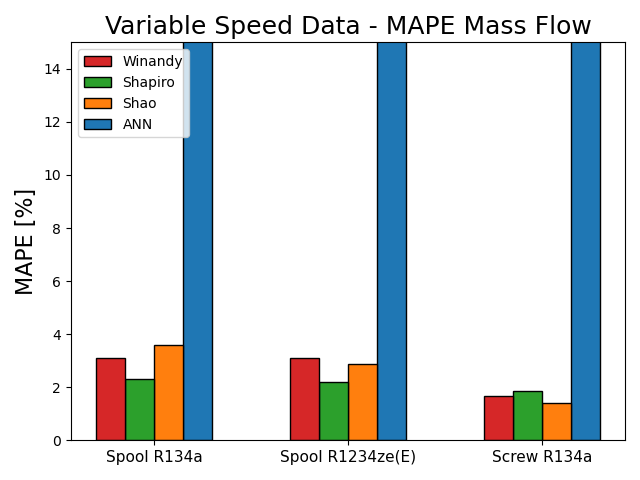
\includegraphics[width=0.7\linewidth]{mdot_vspeed.png}
\caption{Showing mass flow rate results under modulation testing. (Errors for ANN Spool R134a, ANN Spool R1234ze(E), and ANN Screw R134a are: 19.9\%, 19.6\%, 25.2\% respectively.)}
\label{fig:mdot_vspd}
\end{figure}
\FloatBarrier

Shown in Figure \ref{fig:mdot_vspd}, the testing results for modulation situations show the Winandy, Popovic and Shapiro, and the Shao model capture mass flow rate at MAPE's less than 5\%. This provides good indication that the aforementioned models could be used to predict mass flow rate at conditions outside the bounds of their training data. The ANN model produced errors around 20\% and performs poorly when tested at modulation scenarios. The errors achieved for the AHRI model are not shown on the modulation bar plot since the screw compressor data did have ten data points at constant superheat and speed to train the model's coefficients. The errors achieved for spool compressor mass flow rate using R134a and R1234ze(E) when running the AHRI model were 20.7\% and 20.3\%, respectively. 


\begin{figure}[!h]
\centering
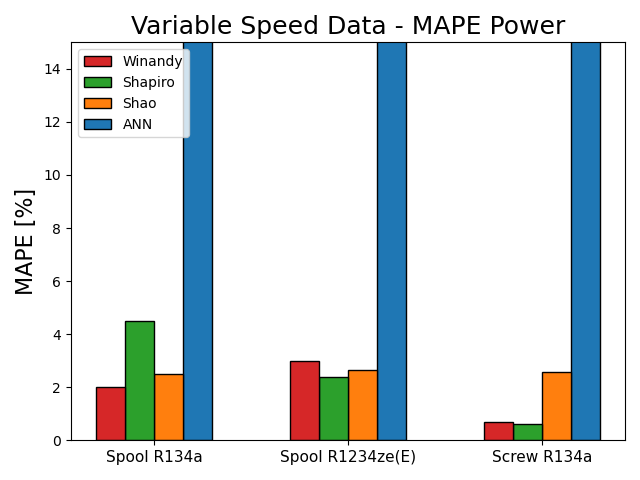
\includegraphics[width=0.7\linewidth]{power_vspeed.png}
\caption{Power results under modulation testing. (Errors for ANN Spool R134a, ANN Spool R1234ze(E), and ANN Screw R134a are: 19.1\%, 20.4\%, 20.6\% respectively.}
\label{fig:power_vspd}
\end{figure}
\FloatBarrier

Shown in Figure \ref{fig:power_vspd}, the results for power prediction under modulation scenarios were similar to that of mass flow rate. The Winandy, Popovic and Shapiro, and Shao model performed under 5\% MAPE. The ANN model again performs at MAPE's around 20\% for power prediction when tested at modulation scenarios. Similar to the mass flow rate, the AHRI model is not shown on the graph for power prediction. The errors achieved for power prediction using the AHRI model and tested with the spool compressor using R134a and R1234ze(E) were  20.2\% and 21.4\%, respectfully.

\subsection{Extrapolation}
Figures \ref{fig:mdot_extrp} and \ref{fig:power_extrp} are bar charts representing the MAPE of model predicted results for each of the models using the three modulation data sets described in Section \ref{sec:extra} with results summarized in Table \ref{Tab:extrp_mdot_results}. 

\begin{figure}[!h]
\centering
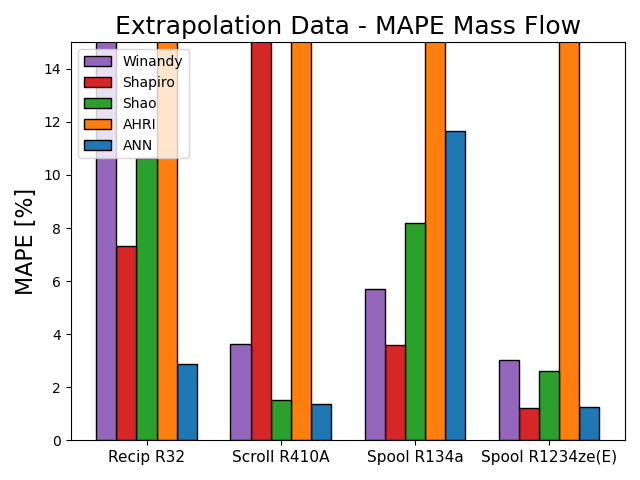
\includegraphics[width=0.7\linewidth]{mdot_extrp.png}
\caption{Mass flow rate results at extrapolation scenarios for all models.}
\label{fig:mdot_extrp}
\end{figure}
\FloatBarrier

\begin{table}[h]
\caption{Mass flow rate MAPE's under extrapolation scenarios.}
\label{Tab:extrp_mdot_results}
\begin{center}
\resizebox{0.8\textwidth}{!}{
\begin{tabular}{c c c c c c}
\hline
\hline
\textbf{Data Set} &  \multicolumn{4}{c}{\textbf{Model MAPE - Mass Flow}} \\
\hline
\- & Winandy   & Popovic \& Shapiro  & Shao & AHRI  & ANN \\
\hline
\textbf{Recip. R32}  & 23.3\%  & 7.3\%  & 10.7\% & 45.1\% & 2.9\% \\
\textbf{Scroll R410A}  & 3.6\%  & 19.3\%  & 1.5\% & 6.4e+5\% & 1.4\% \\
\textbf{Spool R134a}  & 5.7\%  & 3.6\%  & 8.2\% & 6.0e+6\% & 11.9\% \\
\textbf{Spool R1234ze(E)}  & 3.0\%  & 1.2\%  & 2.6\% & 3.5e+6\% & 1.3\% \\
\hline
\hline
\end{tabular}
}
\end{center}
\end{table}

Shown in Figure \ref{fig:mdot_extrp}, results show that mass flow rate extrapolation is captured by the semi-empirical models, given that they do predict the compressor technology. The Winandy model performs below 6\% MAPE for the scroll and spool compressor technologies. The model extrapolated with two different refrigerant data sets for the spool compressor. The model did not capture reciprocating compressor performance. The Popovic and Shapiro model extrapolated below 8\% MAPE for the compressor technologies that it predicted. This model however, did not capture scroll compressor technology but performed better at extrapolating spool compressor data than reciprocating data, the latter of which the model was derived initially to predict. The ANN model extrapolated below 3\% MAPE except in the case of the spool compressor utilizing R134a. The Shao model performed well when ran with scroll and the spool R1234ze(E) data, however extrapolation errors rose to 8.2\% and 10.7\% MAPE for the reciprocating and spool R134a data respectively. The AHRI model did not perform adequately when extrapolating as can be seen by the errors rising from 45.\% to 6.0e+6.

% ------------------------------------------------------
% ------------------------------------------------------
\begin{figure}[!h]
\centering
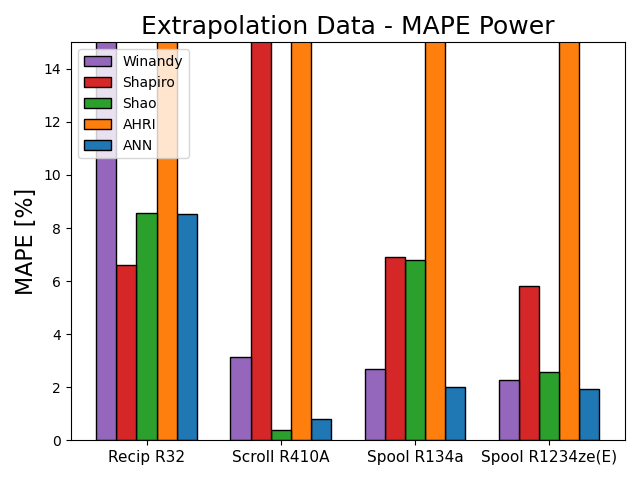
\includegraphics[width=0.7\linewidth]{power_extrp.png}
\caption{Power results under extrapolation testing for all models.}
\label{fig:power_extrp}
\end{figure}
\FloatBarrier

\begin{table}[h]
\caption{Power MAPE's for extrapolation scenarios.}
\label{Tab:extrp_pwr_results}
\begin{center}
\resizebox{0.8\textwidth}{!}{
\begin{tabular}{c c c c c c}
\hline
\hline
\textbf{Data Set} &  \multicolumn{4}{c}{\textbf{Model MAPE - Power}} \\
\hline
\- & Winandy   & Popovic \& Shapiro  & Shao & AHRI  & ANN \\
\hline
\textbf{Recip. R32}  & 16.4\%  & 6.6\%  & 8.6\% & 27.5\% & 8.5\% \\

\textbf{Scroll R410A}  & 3.1\%  & 3.4e+3\%  & 0.4\% & 9.0e+5\% & 0.8\% \\

\textbf{Spool R134a}  & 2.7\%  & 6.9\%  & 6.8\% & 6.7e+6\% & 1.9\% \\

\textbf{Spool R1234ze(E)}  & 2.3\%  & 5.8\%  & 2.6\% & 6.3e+4\% & 1.9\% \\

\hline
\hline
\end{tabular}
}
\end{center}
\end{table}

Shown in Figure \ref{fig:power_extrp}, since the mass flow rate results are used in the power prediction for the Winandy and Popovic and Shapiro models, it can be expected that when either model doesn't predict the mass flow rate adequately, the power formulation will suffer. This is the case for the Winandy model predicting reciprocating compressor power requirements and the Shapiro and Popovic model predicting scroll compressor power requirements under envelope extrapolation scenarios. When the Winandy model predicts the compressor technology, it extrapolates below 4\% MAPE. The Popovic and Shapiro model extrapolates below 7\% MAPE. The Shao model extrapolated below 9\% MAPE for all cases while the ANN model performed under 2\% MAPE for cases except that of the reciprocating data in which it performed at 8.5\% MAPE. The AHRI model did not extrapolate adequately. It produced errors between 27.5\% and 6.7e+6\% MAPE. 

\subsection{Variable Superheat}
\lcom{copy what I did above}{Look at how I added information to the above sections and please update this section to be consistent. It is critical to introduce each technical figure and discuss what is in it before discussing results.}

\begin{figure}
\centering
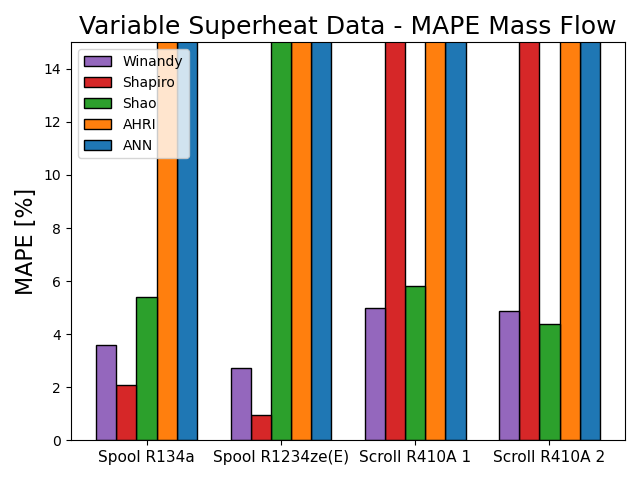
\includegraphics[width=0.75\linewidth]{mdot_vspr.png}
\caption{Mass flow rate results under variable superheat testing.}
\label{fig:mdot_vspr}
\end{figure}
\FloatBarrier

\begin{table}[h]
\caption{Mass flow rate results for variable superheat scenarios.}
\label{Tab:vspr_mdot_results}
\begin{center}
\resizebox{0.8\textwidth}{!}{
\begin{tabular}{c c c c c c}
\hline
\hline
\textbf{Data Set} &  \multicolumn{4}{c}{\textbf{Model MAPE - Mass Flow Rate}} \\
\hline
\- & Winandy   & Popovic \& Shapiro  & Shao & AHRI  & ANN \\
\hline
\textbf{Spool R134a}  & 3.6\%  & 2.1\%  & 5.4\% & 2.9e+5\% & 25.5\% \\
\textbf{Spool R1234ze(E)}  & 2.7\%  & 1.0\%  & 42.2\% & 6.0e+7\% & 20.9\% \\
\textbf{Scroll R410A 1}  & 5.0\%  & 20.1\%  & 5.8\% & 6.6e+5\% & 21.2\% \\
\textbf{Scroll R410A 2}  & 4.9\%  & 19.3\%  & 4.4\% & 6.6e+5\% & 18.6\% \\
\hline
\hline
\end{tabular}
}
\end{center}
\end{table}

The mass flow rate for variable superheat scenarios is best predicted by the Winandy model. The Shapiro and Popovic model performs well for the compressor technology it does predict, it performs under 2.5\% MAPE for the spool data sets. The Shao model predicts mass flow under 6\% for all cases except the spool compressor data set using R1234ze(E). As can be seen from the bar chart and table, the AHRI model does noit predict mass flow rate at variable superheat condition adequately. There exists a superheat correction factor for the model, however it is not applied in the present study. The ANN model predicts mass flow rate at a MAPE above 20\% for all situations and yielded inadequate results.  

\begin{figure}
\centering
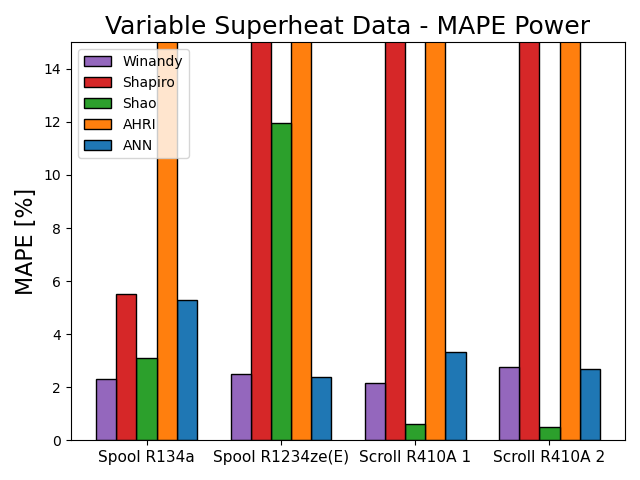
\includegraphics[width=0.7\linewidth]{power_vspr.png}
\caption{Power results under variable superheat testing.}
\label{fig:power_vspr}
\end{figure}
\FloatBarrier

\begin{table}[h]
\caption{Power results for variable superheat scenarios.}
\label{Tab:vspr_pwr_results}
\begin{center}
\resizebox{0.8\textwidth}{!}{
\begin{tabular}{c c c c c c}
\hline
\hline
\textbf{Data Set} &  \multicolumn{4}{c}{\textbf{Model MAPE - Power}} \\
\hline
\- & Winandy   & Popovic \& Shapiro  & Shao & AHRI  & ANN \\
\hline
\textbf{Spool R134a}  & 2.3\%  & 5.5\%  & 3.1\% & 5.8e+5\% & 5.3\% \\
\textbf{Spool R1234ze(E)}  & 2.5\%  & 2.4\%  & 11.9\% & 1.6e+6\% & 2.4\% \\
\textbf{Scroll R410A 1}  & 2.2\%  & 232\%  & 0.6\% & 9.2e+5\% & 3.3\% \\
\textbf{Scroll R410A 2}  & 2.8\%  & 372\%  & 0.5\% & 9.0e+5\% & 2.7\% \\
\hline
\hline
\end{tabular}
}
\end{center}
\end{table}

Power results show that the Winandy model performed best at predicting variable superheat power consumption. The model performed below 3\% MAPE for all data sets. The Shapiro and Popovic model performed under 6\% MAPE for the technologies it predicted. The errors resulting from the scroll power prediction were above 200\% MAPE. The Shao model performed well at power prediction for the data sets resulting in MAPE's under 3.5\% except for the spool data set using R1234ze(E), where it yielded 11.1\% MAPE. The AHRI model did not perform adequately and gave errors above 5.8e5\%. The ANN model performed better at power prediction than mass flow rate prediction for variable superheat scenarios. The model gave MAPE's below 5.5\% for all data sets it was tested with. 


\section{Discussion}

The Winandy model failed to predict reciprocating compressor data while the Popovic and Shapiro model did not predict scroll compressor data. The semi-empirical models do extrapolate and capture modulation provided the model first predicts the data. The AHRI model does not extrapolate or capture modulation adequately. The ANN model does extrapolate to a reasonable level, however it does not predict variable speed performance. The Shao model captures extrapolation and modulation to a reasonable level, but requires variable speed data in its training data pool. The Shao model was derived for capturing variable speed performance, therefore it is not unreasonable to expect it to perform well in modulation testing.

The semi-empirical models (Winandy model and Popovic and Shapiro model) performed adequately in extrapolation and modulation scenarios. Given that the model predicted the compressor technology, the highest MAPE for mass flow rate came from the Shapiro and Popovic model at 7.3\%. For power prediction the same model recorded the highest error, which was 6.9\%. The more empirical Shao model gave promising results for mass flow rate and power prediction in modulation scenarios, however, mixed results were achieved in extrapolation testing where resulting MAPE's ranged from 0.4\% to 42.2\%. The AHRI formulation performed the worst in modulation and extrapolation scenarios. Results show that the model should not be used in modulation scenarios or beyond the bounds of its' training data. The ANN model has performed poorly in modulation scenarios where errors above 19\% were recorded in all data sets. In extrapolation scenarios, results were mixed with MAPE's between 0.8\% and 25.5\%. 

From these results some conclusions can be made regarding the performance of the semi-empirical and empirical models.
\begin{itemize}
\item The Winandy model, as tested, will capture extrapolation and modulation in scroll, screw, and spool compressors
\end{itemize}
\begin{itemize}
\item The Winandy model outperforms the Shapiro and Popovic model when compared head to head
\end{itemize}
\begin{itemize}
\item The ANN model cannot predict performance during compressor modulation, given a constant speed training data set
\end{itemize}
\begin{itemize}
\item The Shao model, even though empirical in nature, will capture modulation scenarios
\end{itemize}
\begin{itemize}
\item The AHRI model will not predict compressor performance under modulation or extrapolation scenarios
\end{itemize}

\subsection{Model Capabilities}

The semi-empirical models yielded more consistent performance at extrapolation and modulation scenarios than the empirical models. The Shao model performed best at modulation scenarios, however as previously mentioned, the model uses variable speed data for training parameters. It does not account for a compression process and only takes data to fit coefficients. Similarly, the ANN and AHRI formulations only require data for tuning parameters. The Winandy model attempts to account for phenomena occurring in the suction line, discharge line, and compression chamber via the isentropic compression assumption and the suction and discharge heat transfer assumptions. The Shapiro and Popovic model does not account for suction and discharge gas heating, but it does model the compression process as polytropic and assumes suction and discharge pressure drops. These two models incorporate more physics into their formulations and the results suggest they are well suited for situations where limited data or model flexibility is desired. \com{It occured to me that the argument for using these approaches includes limited data and/or flexibility}

\subsubsection{Model Limitations}

The five models tested in this work have limitations due to either training data or performance prediction. The training data for a model should require minimal operating conditions and no detailed information derived from comprehensive measurements of the compressor. To this end, the Shao and the Popovic and Shapiro models training data is a limiting factor. Shao requires operating conditions at three different operational speeds to adequately fit the power and mass flow ratios. The Shapiro and Popovic model requires discharge temperature measurements to fit the polytropic exponent to pressure ratio. Limitations in performance prediction are exhibited by each model. The Winandy model did not capture reciprocating compressor performance and the Shapiro and Popovic model did not capture scroll compressor performance. Other models exhibited limitations during specific testing scenarios. The ANN model did not predict predict compressor behavior during modulation testing. The AHRI model exhibited large errors throughout testing. 

\subsection{Future Model Development}

Future work based on the results presented herein will be developing a compressor model to capture multiple compressor technologies and adequately capture modulation and extrapolation. The model will be tested subject to the same methodology as used here. The Winandy model offered good results during testing of the compressors that it predicted. With its performance here and the body of literature showing modifications, it is selected as the basis for future model development.


\section{Conclusions}

\lcom{add more quantitative results to conclusion}{This section does highlight the biggest conclusion, which is the the Winandy model seems like the best candidate to modify moving forward.  However, it does not include anything else.  Add to this section some of the other conclusions, where were models strong/weak and how were they quantified?  Keep in mind, that for most people skimming your paper, they will read the abstract, introduction, and conclusion, if they don't like what they see there they won't read the rest of it. }

The present work studied the extrapolation and modulation capabilities of select semi-empirical compressor models. Data sets selected for model testing were of high fidelity to ensure model prediction is accurate to measured data instead of manufacture published data. Data sets were split to enable training model parameters at constant conditions then test model with data outside that of the training data. Four different data sets were identified and used: the training data set, envelope extrapolation data set, variable superheat data set, and variable speed data set. Models were trained using the training data set then tested at the others to record performance. Based on the results, the semi-empirical models outperform the empirical models when considering all aspects desired by the author. These were: limited training data, low computational cost, and accurate performance at extrapolation and modulation scenarios. The model proposed by \cite{Winandy_recip} is chosen as a formulation with promising attributes for future model development. As cited in the literature survey, this formulation has been modified to capture a range of technologies and will be the basis for a new model desired to capture multiple compressor technologies and exhibit strong extrapolation and modulation capabilities.

\section{Acknowledgment}
The authors would like to acknowledge the Center for Integrated Building Systems, an Industry/University cooperative research center at Oklahoma State University for funding this study. They would also like to thank Joe Orosz of Torad Engineering for his valuable mentorship and feedback.

\newpage
\FloatBarrier
\bibliographystyle{agsm}

\bibliography{library}

\newpage
\appendix


\end{document}